\begin{figure*}[t]
\centering
\resizebox{\textwidth}{!}{%
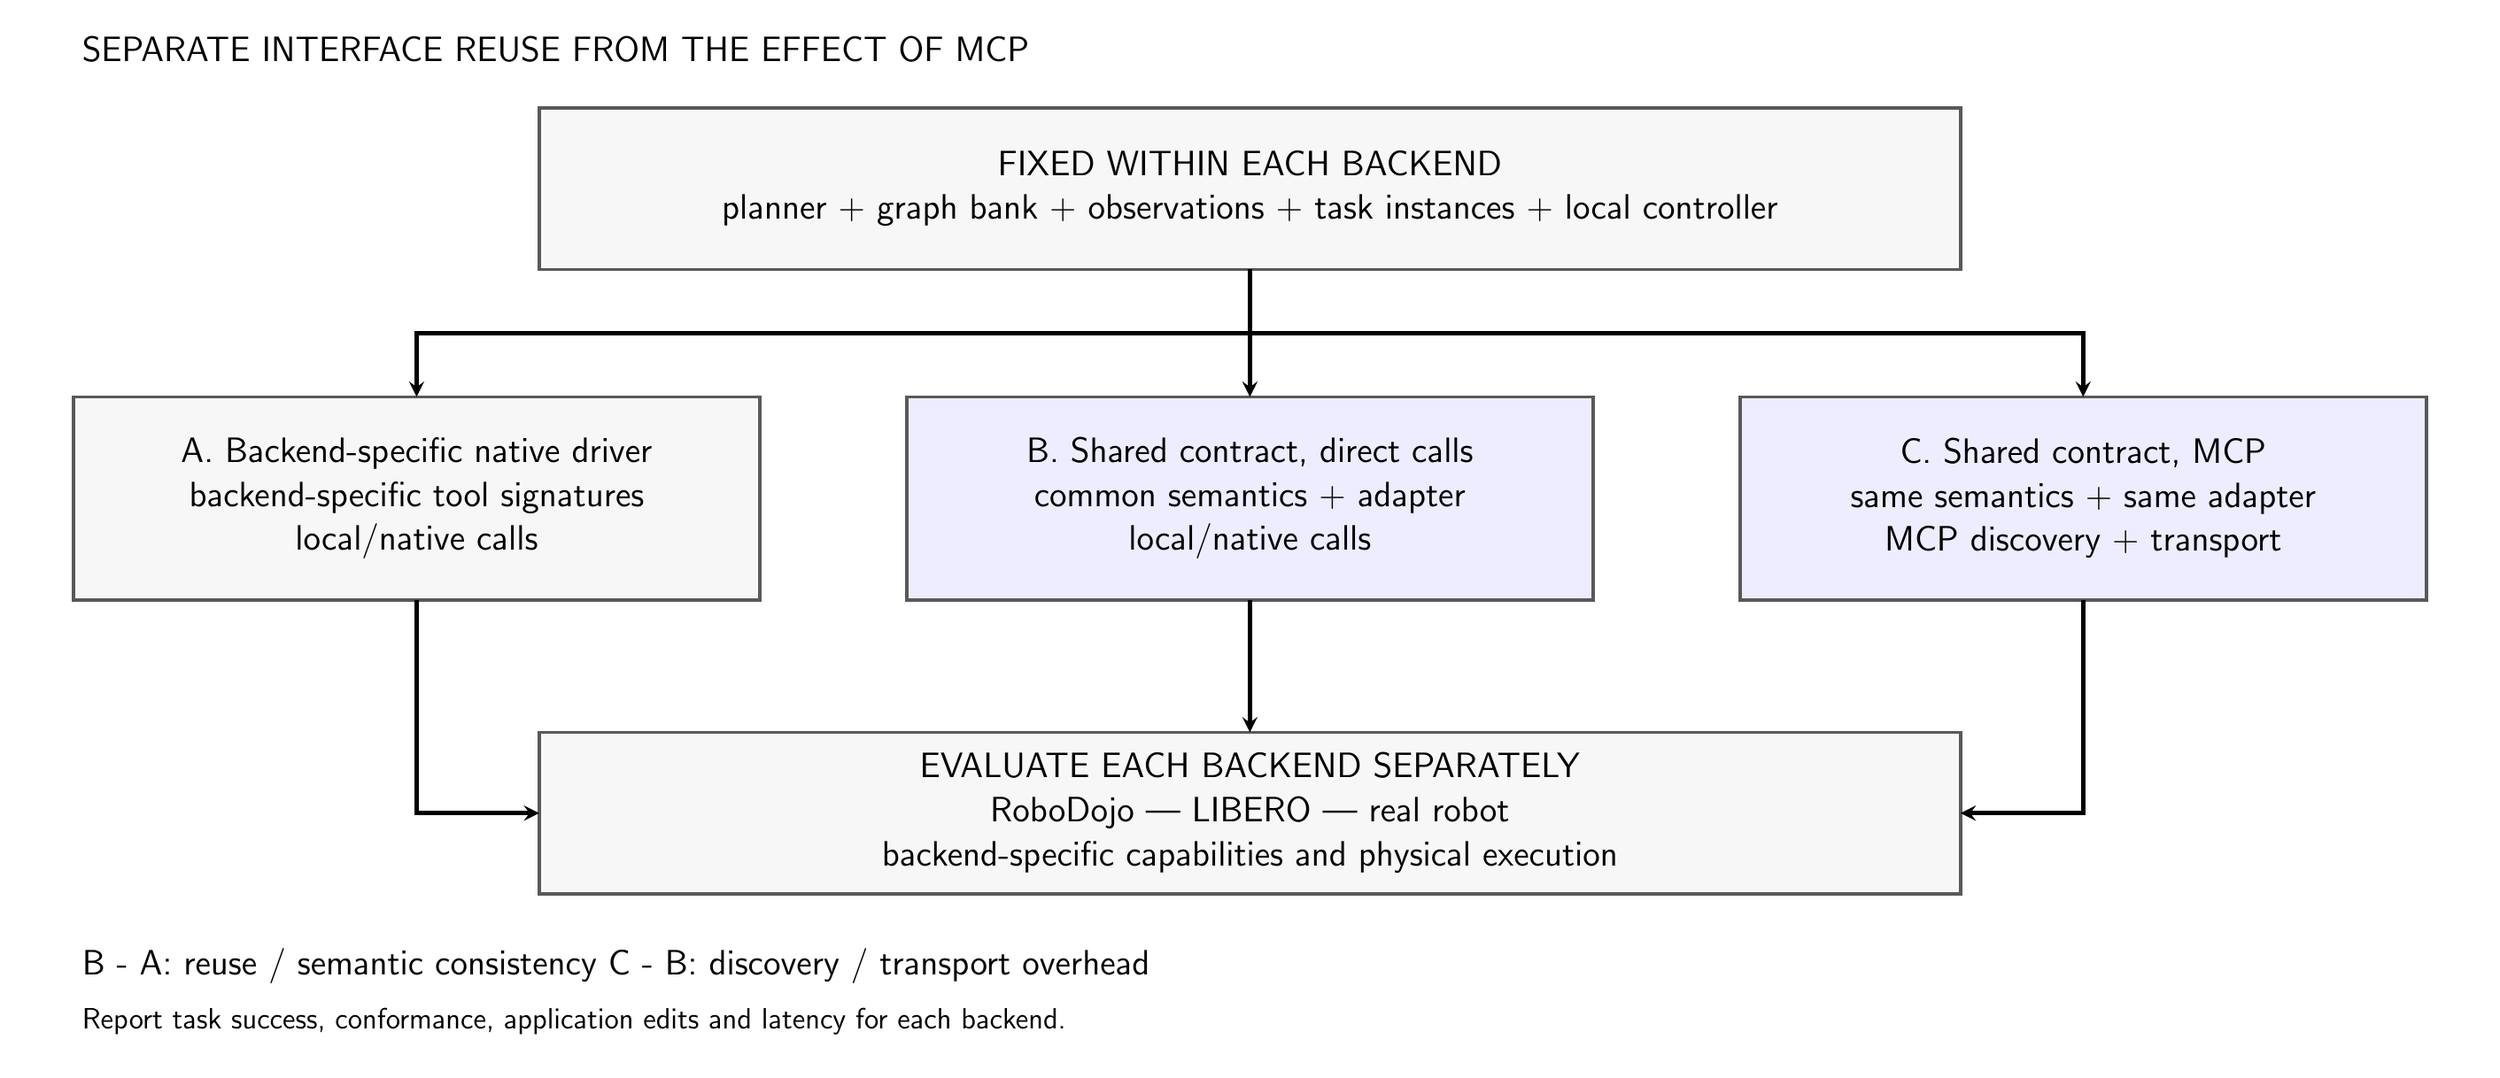
\begin{tikzpicture}[x=1pt,y=1pt,>=stealth]
\path[use as bounding box] (0,0) rectangle (1000,420);
\node[draw=black!65,fill=black!3,line width=1.3pt,minimum width=580pt,minimum height=66pt,text width=568pt,inner sep=4pt,align=center,font=\sffamily\fontsize{15}{18}\selectfont] (shared) at (500.0,353.0) {FIXED WITHIN EACH BACKEND\\planner + graph bank + observations + task instances + local controller};
\node[draw=black!65,fill=black!3,line width=1.3pt,minimum width=280pt,minimum height=83pt,text width=268pt,inner sep=4pt,align=center,font=\sffamily\fontsize{15}{18}\selectfont] (a) at (160.0,226.5) {A. Backend-specific native driver\\backend-specific tool signatures\\local/native calls};
\node[draw=black!65,fill=blue!7,line width=1.3pt,minimum width=280pt,minimum height=83pt,text width=268pt,inner sep=4pt,align=center,font=\sffamily\fontsize{15}{18}\selectfont] (b) at (500.0,226.5) {B. Shared contract, direct calls\\common semantics + adapter\\local/native calls};
\node[draw=black!65,fill=blue!7,line width=1.3pt,minimum width=280pt,minimum height=83pt,text width=268pt,inner sep=4pt,align=center,font=\sffamily\fontsize{15}{18}\selectfont] (c) at (840.0,226.5) {C. Shared contract, MCP\\same semantics + same adapter\\MCP discovery + transport};
\node[draw=black!65,fill=black!3,line width=1.3pt,minimum width=580pt,minimum height=66pt,text width=568pt,inner sep=4pt,align=center,font=\sffamily\fontsize{15}{18}\selectfont] (backends) at (500.0,98.0) {EVALUATE EACH BACKEND SEPARATELY\\RoboDojo  |  LIBERO  |  real robot\\backend-specific capabilities and physical execution};
\draw[->,line width=1.7pt] (500,320) -- (500,294) -- (160,294) -- (160,268);
\draw[->,line width=1.7pt] (500,320) -- (500,268);
\draw[->,line width=1.7pt] (500,294) -- (840,294) -- (840,268);
\draw[->,line width=1.7pt] (160,185) -- (160,98) -- (210,98);
\draw[->,line width=1.7pt] (500,185) -- (500,131);
\draw[->,line width=1.7pt] (840,185) -- (840,98) -- (790,98);
\node[anchor=base west,font=\sffamily\fontsize{15}{18}\selectfont] at (20,405) {SEPARATE INTERFACE REUSE FROM THE EFFECT OF MCP};
\node[anchor=base west,font=\sffamily\fontsize{15}{18}\selectfont] at (20,32) {B - A: reuse / semantic consistency     C - B: discovery / transport overhead};
\node[anchor=base west,font=\sffamily\fontsize{13}{18}\selectfont] at (20,10) {Report task success, conformance, application edits and latency for each backend.};
\end{tikzpicture}}
\caption{Proposed interface comparison on RoboDojo, LIBERO and a real robot. Within each backend, all three modes use the same planner, graph bank, observations, task instances and local controller. Mode A uses a backend-specific native driver. Mode B routes calls through the proposed common capability, observation, action and receipt contract. Mode C exposes exactly the same contract and adapter through MCP. B versus A tests semantic normalization and reuse; C versus B tests the incremental effect of protocol discovery and transport, including its overhead. The three backend names denote planned validation targets, not completed integrations. A shared contract does not make backend physics or capabilities identical.}
\label{fig:platform}
\end{figure*}
